\documentclass[12pt]{article} %Define o documento como um artigo
\usepackage[portuguese]{babel} %Define a linguagem do documento como português
\usepackage[utf8]{inputenc} %Para entender todos os caracteres
\usepackage[a4paper, portrait, margin=2cm]{geometry} %Define a pagina como sendo tamanho A4, em modo retrato, com margem de 2 cm
\usepackage{dirtytalk} %Para usar o \say, que coloca aspas na frase
\usepackage{indentfirst} %Para indentar o primeiro parágrafo 
\setlength{\parindent}{2em} %Define o tamanho da indentação
\usepackage{soul} %Para fazer texto tachado
\usepackage{pgfplots} %Pacote de graficos
\pgfplotsset{compat=1.9}
\usepgfplotslibrary{statistics}
\usepackage{pgf-pie} %Graficos de pizza
\usepackage{wrapfig} %Figuras em volta de texto
\usepackage{tabularx} %Tabelas de qualquer tamanho
\usepackage{amsmath} %Biblioteca de integrais
\usepackage{mathtools} 
\usepackage{esint} %Biblioteca de integrais ciclicas
\usepackage{titlesec}
\usepackage{subcaption}
\usepackage{systeme}
\usepackage[spaces,hyphens]{url}
\usepackage{float}
\usepackage{multirow}
\usepackage{graphics}

\begin{document}

    \begin{titlepage}
        \begin{center}
            
            \LARGE{\textbf{Métodos Numéricos e Aplicações - MAP3121}}
            
            \vspace{20pt}
            
            \LARGE{\textbf{Exercício-Programa 2}}
            
            \vspace{200pt}
            
            \LARGE{\textbf{Autovalores e Autovetores de Matrizes Reais Simétricas}}
            
            \vspace{40pt}
            
            \LARGE{\textbf{O Algoritmo QR}}
            
            \vspace{80pt}
            
            \begin{flushright}
                \Large{\textsc{Pedro H. G. Cazelatto - NUSP 11261090}}
            \end{flushright}
            
            \vfill
            
            São Paulo - SP
            
            21/07/2021
            
        \end{center}
    \end{titlepage}
    
    \section{Introdução}
    
        O programa foi desenvolvido em linguagem C para que sua execução fosse mais rápida. Para facilitar o entendimento inicial, realizei alguns \textit{scripts} no \textit{software} Octave conforme lia o enunciado, transformando o \say{matematiquês} em um código simples executável, o que ajudou no planejamento de funções, para minimizar repetição de código, e também na depuração do código final, pois me permitia conferir os valores.
        
        \vspace{\baselineskip}
        
    \section{O problema}
        
        No EP1 foi desenvolvido um algoritmo que calculava autovalores e autovetores de uma dada matriz tridiagonal simétrica, que é um caso muito específico. Para aumentar a abrangência, neste EP2 usaremos transformações de Householder para levar uma matriz real simétrica a uma matriz tridiagonal, para aplicarmos no algoritmo já desenvolvido de cálculo de autovalores e autovetores.
        
        A transformação de Householder é realizada através da multiplicação da matriz de transformação pela matriz a ser transformada, porém é um processo ruim de escalar, pois multiplicar matrizes tem ordem $O(n^3)$. Para isso, foi descrito uma versão mais rápida e mais específica, que é aplicada a vetores da matriz de entrada, diminuindo a ordem para $O(n^2)$.
        
        Da matriz transformada, é possível extrair os autovalores e autovetores com o algoritmo QR já desenvolvido, porém os autovetores da transformada precisam ser multiplicados pela matriz $H^T$ para que se tornem os autovalores da matriz não transformada.
        
        \vspace{\baselineskip}
        
    \section{Primeiros programas}
        
        Assim como no EP1, me dei ao trabalho de fazer um \textit{script} no Octave para depuração e entendimento do código, pelo mesmo motivo de ter feito no EP1: o Octave fornece um degrau entre a explicação textual do enunciado e a complexidade de um código em C. Apesar de levar mais tempo, o aprendizado foi significativamente facilitado.
        
        \subsection{A repaginada}
            
            No EP1, desenvolvi o código inteiro usando matrizes pois acreditei que não faria muita diferença. Após ver muita discussão entre alunos e professores, decidi fazer a melhoria: repensei o código do algoritmo QR com deslocamento espectral para funcionar com apenas três vetores, cada um correspondendo a uma das diagonais.
            
            Fiquei surpreso quando fiz o primeiro teste com uma matriz 32x32 e o tempo de execução foi 10 vezes maior, mas para o algoritmo otimizado. Comecei a procurar erros pelo código mas estava totalmente correto. Então veio a realização: a medição de tempo foi feita executando os \textit{scripts} no Octave, que utiliza paralelismo para multiplicar matrizes, acelerando muito o processamento. Creio que seja um dos motivos para não ter otimizado o código antes, no EP1.
            
            Após a descoberta, resolvi fazer o teste em C, que foi onde a diferença ficou clara (e correta). O algoritmo sem a otimização levava 20 segundos para processar uma matriz 64x64, enquanto o otimizado levava menos de um segundo.
            
        \subsection{O novo algoritmo}
            
            Com o algoritmo QR otimizado para rapidez, resolvi já fazer o algoritmo das transformações de Householder otimizado. Para cada valor de $i$, o vetor $\omega$ é calculado, e com ele as linhas e colunas da matriz de entrada são transformadas, assim como a matriz $Ht$, que iniciou como uma matriz identidade, e servirá para o cálculo dos autovetores.
            
            \begin{figure}[H]
                \centering
                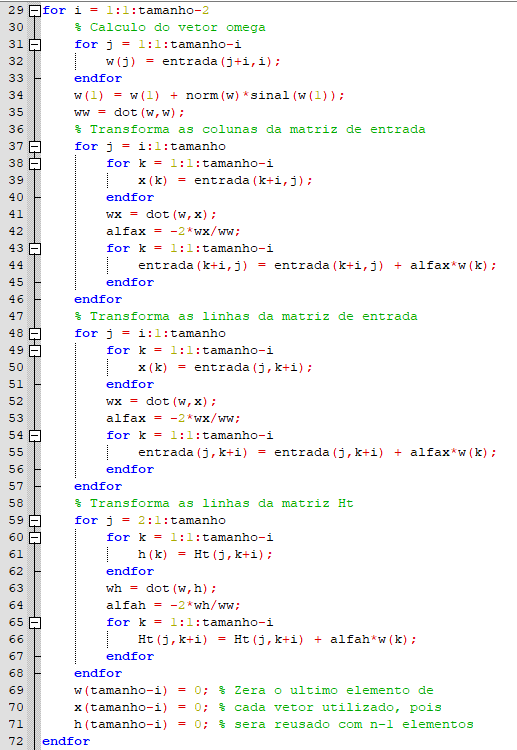
\includegraphics[width=0.75\linewidth]{Tridiagonalizacao.png}
                \caption{Transformação tridiagonalizadora de Householder}
                \label{fig:tridiag}
            \end{figure}
            
            \vspace{\baselineskip}
            
    \section{Traduzindo para C}
        
        Após diversos testes bem sucedidos no Octave, além das funções preexistentes do primeiro código, criei também uma função para calcular a norma de um vetor de tamanho $n$ e outra para calcular o produto escalar de dois vetores de tamanho $n$. Criei uma função separada também para tridiagonalização da matriz, para evitar repetição massiva de código.
        
        A função \textit{main} é responsável por perguntar ao usuário qual teste ele deseja executar, pedir os parâmetros necessários para tal execução, imprimir na tela os dados iniciais do teste e seus resultados e coordenar as diversas funções já citadas de modo a executar o teste com perfeição.
        
        Como foi passado a nós arquivos contendo valores para facilitar a entrada, adicionei a opção do usuário passar o nome do arquivo para que o programa faça a leitura.
        
        \vspace{\baselineskip}
        
    \section{Testes}
        
        O objetivo principal deste exercício-programa é calcular modos de vibração de uma treliça, a partir da matriz de rigidez total dos nós livres. Entretanto, para começar de maneira mais leve, foi pedido alguns testes com matrizes reais mais simples.
        
        \subsection{Com matrizes}
            
            O primeiro dos testes é com uma matriz 4x4, descrita na figura \ref{fig:testeA}, que mostra a entrada por arquivo e as saídas do programa. Pode-se confirmar que o programa funciona corretamente fazendo a conta:
            
            $$ \text{entrada}*\text{autovetor} = \text{autovalor}*\text{autovetor} $$
            
            \begin{figure}[H]
                \centering
                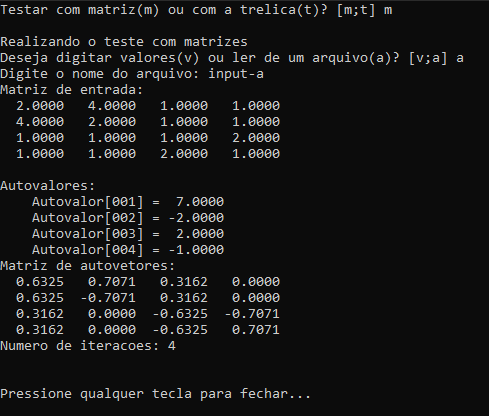
\includegraphics[width=0.6\linewidth]{TesteA.png}
                \caption{Teste A}
                \label{fig:testeA}
            \end{figure}
            
            Para o segundo teste foi passada uma matriz 20x20, que não colocarei a foto aqui no relatório pois sua saída não cabe em minha tela de maneira legível, tampouco em uma única foto, mas basta entrar com o arquivo \say{input-b} que você verá que ela também funciona perfeitamente.
            
            \vspace{\baselineskip}
            
        \subsection{Com treliças}
            
            Para o teste principal foi passado um arquivo contendo a descrição de uma treliça, indicando os nós das pontas de cada barra, constantes do material das barras e outros valores. A partir disso, o programa monta a matriz de rigidez total da treliça, encontra uma matriz semelhante que seja simétrica e calcula os autovalores e autovetores. Novamente, não coloquei uma foto da saída pois a matriz resultante é 24x24, o que a torna ilegível em minha tela.
            
            A raiz quadrada dos autovalores correspondem às frequências de vibração da treliça, enquanto os autovetores multiplicados pela matriz de massas elevada a $-0,5$ correspondem aos modos de vibração, ou seja, a amplitude da vibração de cada nó. As 5 menores frequências e seus respectivos modos de vibração são salvos em um arquivo "saidaTesteTrelica.txt" assim que o programa executar uma vez o teste com a treliça.
            
            Junto com os arquivos enviados encontram-se alguns GIFs da treliça proposta no enunciado se movendo. Contudo, como a rigidez da treliça é muito grande, seus movimentos são muito pequenos, de modo que para a vibração ser perceptível multipliquei todas as intensidades por $1000$. A variável do tempo não está sincronizada com o tempo real, porém na animação com duas frequências ambas usam a mesma variável temporal, ou seja, a relação de tempo entre elas é constante.
            
            Como C não possui uma biblioteca para criação de gráficos nativa, utilizei o \textit{software online} GeoGebra\footnote{https://www.geogebra.org/classic} para realizar as animações. Os arquivos produzidos também foram enviados na pasta: \say{Trelica1000w1.ggb} mostra a treliça com movimentos amplificados por 1000 na frequência $\omega_1$ (a menor), \say{Trelica1000w2.ggb} mostra a treliça com movimentos amplificados por 1000 na frequência $\omega_2$ (a segunda menor) e \say{Trelica1000w1w2.ggb} mostra a treliça com movimentos amplificados por 1000 na frequência $\omega_1$ e $\omega_2$ (as duas menores juntas).
            
            \vspace{\baselineskip}
            
    \section{Conclusão}
        
        Ao longo de minha jornada pelos exercícios-programa, percebi a diferença que há na otimização de um algoritmo, mesmo para linguagens rápidas como C. A apresentação de um problema real como o cálculo de frequências de vibração de uma treliça ajudam e muito no entendimento dos exercícios, dando uma motivação mais tangível para nós, engenheiros.
        
\end{document}
